% 第 2 页正文：策略规则、图表、验收对照、迭代历程、局限与附录
\section*{策略规则（champion v2）与执行细节}
规则类型：单阈值二元择时。每日收盘读取温度计总值：$>$80 目标清仓，
$\leq$80 目标满仓；t 日判定、t+1 收盘执行（收盘价为后复权价）；回测起点
温度 6.82 $\leq$80，立即满仓；仓位二元（100\%/0\%），无现金保留与分档。
成本：佣金单边万 3、双边计提；ETF 无印花税；无滑点（或高估收益，见局限）。

\begin{center}
\captionof{figure}{v2 策略与买入持有净值对比（对数轴；粉色区间为 2022 慢熊，
策略与基线回撤重合）}\label{fig:equity}
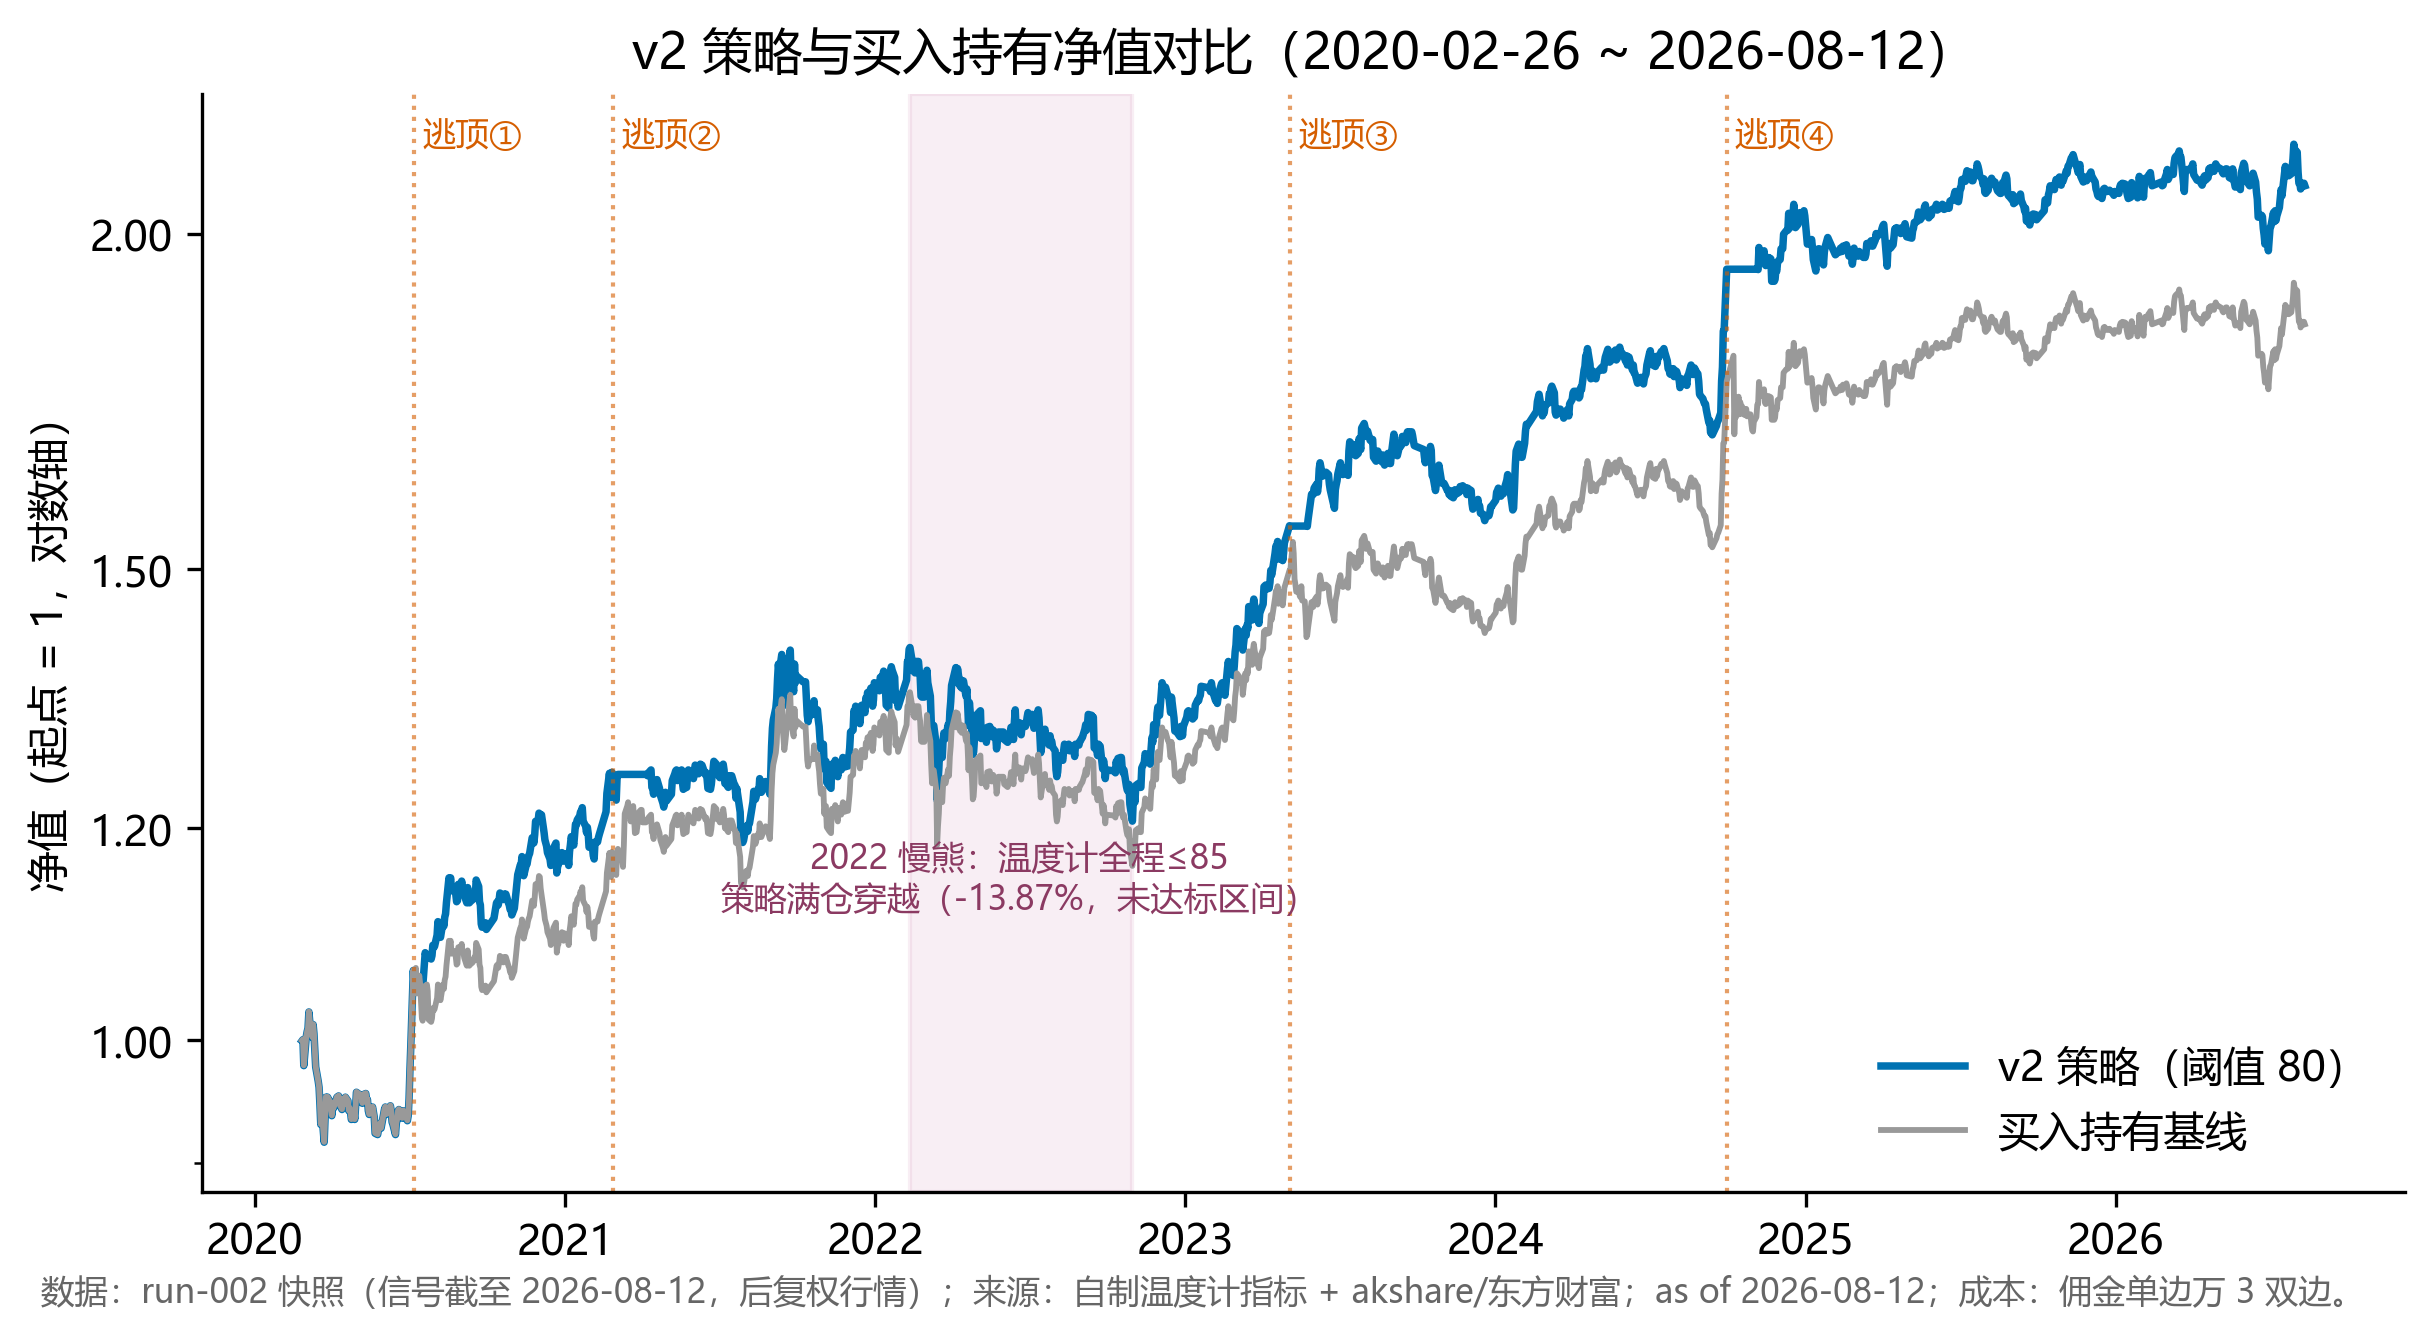
\includegraphics[width=0.86\linewidth]{../figures/fig1_equity.png}
{\footnotesize 来源：run-002 数据快照（信号截至 2026-08-12，后复权行情）；
as of 2026-08-12；成本佣金单边万 3 双边。\par}
\end{center}

\section*{验收对照（task.md 五条标准，对照买入持有基线）}
\begin{center}
\captionof{table}{五条验收标准逐条判定（champion v2，基线同快照重算）}\label{tab:acceptance}
{\footnotesize 判定为确定性代码输出（review/auto\_review.json），LLM 无权更改。\par}
\begin{tabular}{llllc}
\toprule
标准 & 要求 & 基线 & 实际 & 判定 \\
\midrule
1 年化收益 & $\geq$基线$\times$1.05 & 10.42\% & $\geq$10.94\% $\to$ 12.55\% & 达标 \\
2 最大回撤 & $\leq$基线$\times$0.7 & -13.87\% & $\leq$-9.71\% $\to$ -13.87\% & {\color{red}未达标} \\
3 夏普比率 & $\geq$基线$\times$1.2 & 0.8063 & $\geq$0.9676 $\to$ 1.0050 & 达标 \\
4 交易次数 & $\geq$ 10 & --- & 19 & 达标 \\
5 稳健性 & 阈值$\pm$5 结论不反转 & --- & 75--85 五组同判未通过（退化） & 字面达标/实质存疑 \\
\midrule
\multicolumn{5}{l}{综合：五条须全部通过 $\to$ {\color{red}未通过（4/5），如实呈现，不放宽标准}} \\
\bottomrule
\end{tabular}

\end{center}

\section*{三轮迭代历程（假设→证据→裁决）}
\begin{center}
\captionof{table}{run-001/002/003 对照；门禁为确定性数值判定，裁决见各 run critic\_verdict.md}\label{tab:iterations}
{\footnotesize 三 run 共用同一数据快照（SHA-256 一致），"改动净效应"对照成立。\par}
{\small\begin{tabular}{llcccp{3.6cm}}
\toprule
run / 假设 & 规则改动 & 年化/回撤/夏普 & 交易 & 门禁判定 & 被证实/证伪的设计知识 \\
\midrule
run-001 / v1 & 单阈值 85 & 12.21\%/-13.87\%/0.971 & 11 & 未达标（回撤） & 指标只逃顶不防熊 \\
run-002 / v2 & 阈值 85$\to$80 & 12.55\%/-13.87\%/1.005 & 19 & 未达标（回撤） & 调参无解：75--85 回撤全部相同 \\
run-003 / v3 & +MA200 趋势过滤 & 6.53\%/-19.02\%/0.600 & 74 & 未达标（第1/2/3条） & 趋势过滤对低波均值回复品种方向性有害；champion 约束否决 \\
\bottomrule
\end{tabular}
}
\end{center}

过程要点：v1 失败根因（2022 慢熊温度计最高 61.1、全年 0 天 $>$85）在 v2 中得到
"调参无解"的证实（75\textasciitilde{}85 五组回撤清一色 -13.87\%）；v3 结构变更
（H1 批准：叠加 200 日均线趋势过滤）在 2022 年买入每次熊市反弹（全年 -14.6\%
对基线 -3.2\%），回撤反深 5.1 个百分点——同阈值 80 对照 v2 年化 -5.7pp，
champion 单调性约束按设计将其否决。迭代预算 3/5 轮，余 2 轮按"防过拟合单一
样本"主动放弃（H2 裁决）。

\begin{center}
\captionof{figure}{温度计信号与 v2 交易点：卖出全部落在温度尖峰（逃顶有效），
2022 年低位游走无信号（防熊缺位）}\label{fig:temp}
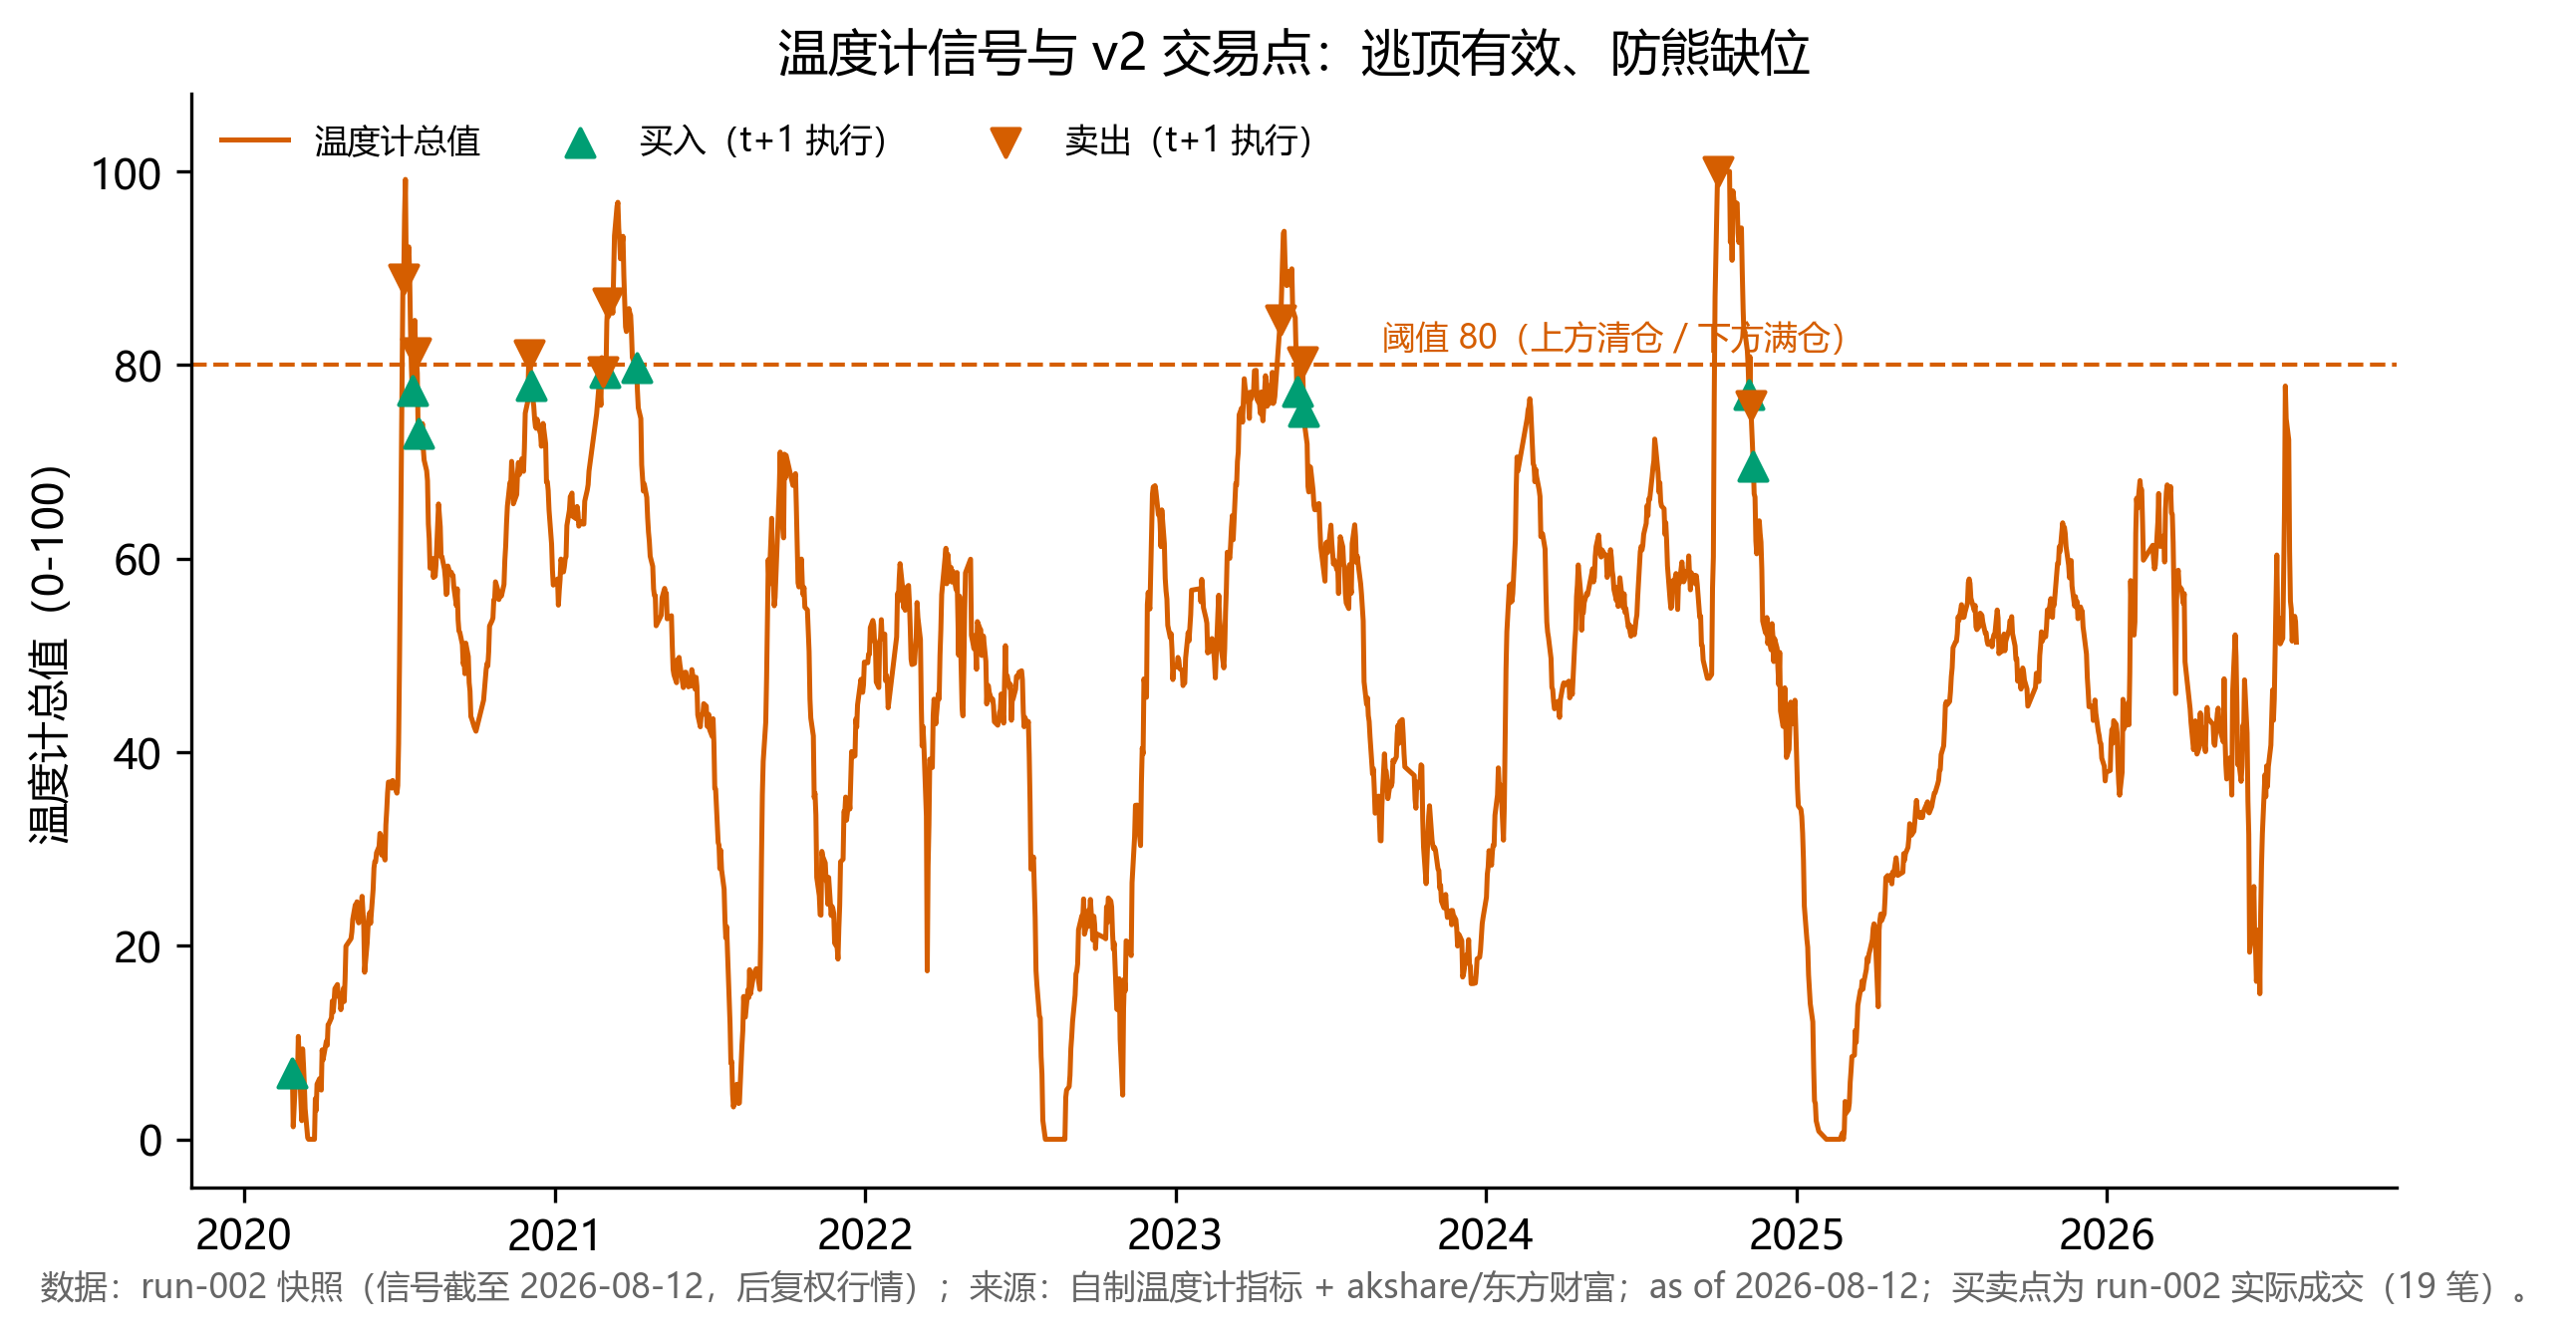
\includegraphics[width=0.86\linewidth]{../figures/fig3_temp_trades.png}
{\footnotesize 来源：run-002 数据快照；买卖点为 19 笔实际成交（t+1 执行）。\par}
\end{center}

\begin{center}
\captionof{figure}{回撤对照：-9.71\% 为验收上限（基线回撤$\times$0.7）；
2022 区间两者回撤曲线重合触底 -13.87\%，第 2 条不达标直证}\label{fig:drawdown}
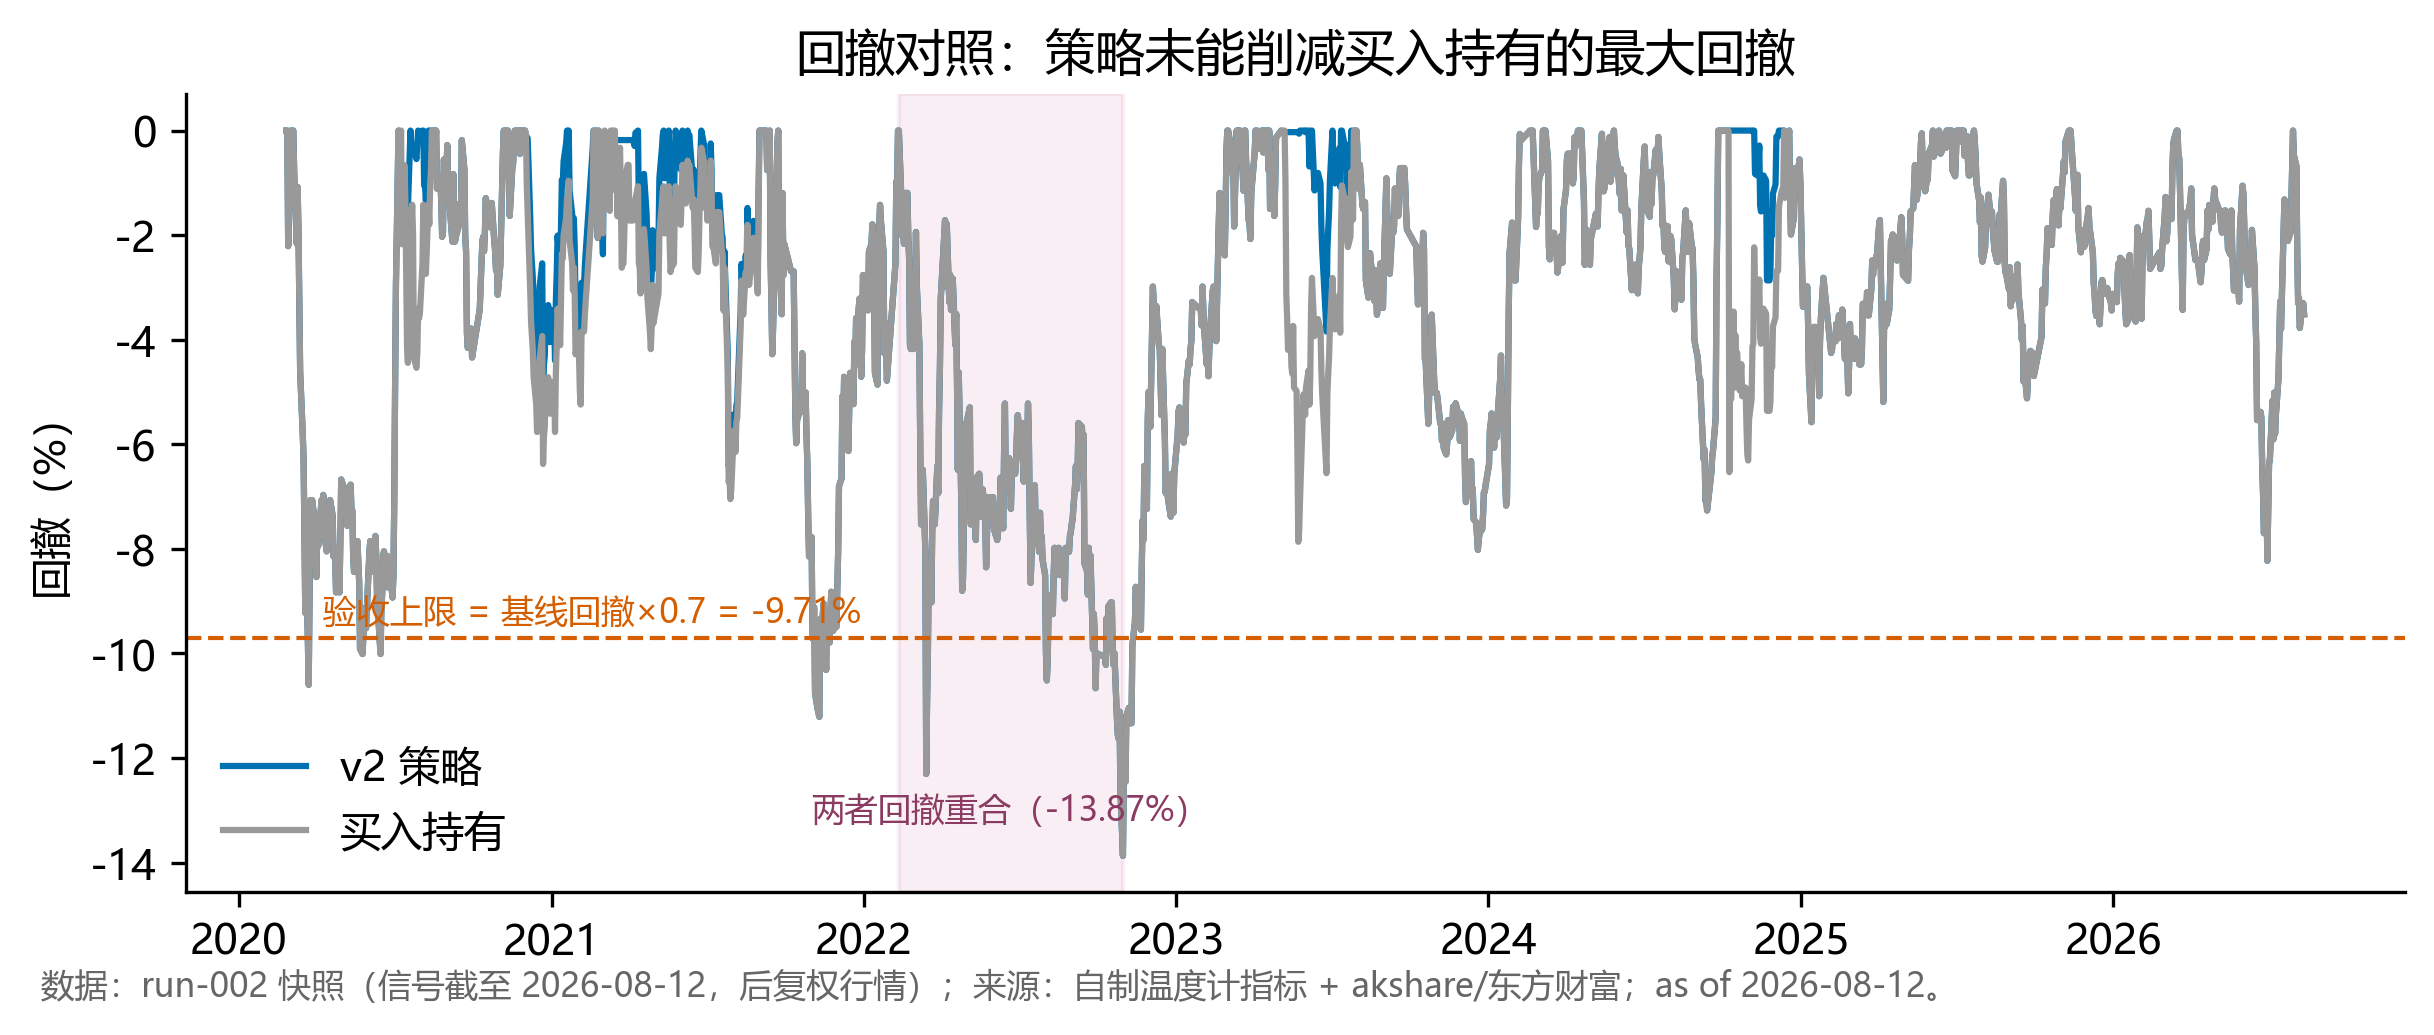
\includegraphics[width=0.8\linewidth]{../figures/fig2_drawdown.png}
{\footnotesize 来源：run-002 数据快照。\par}
\end{center}

\section*{局限与诚实结论}
\begin{itemize}\setlength{\itemsep}{2pt}
  \item \textbf{结论按验收规则为未通过}（4/5）：第 2 条最大回撤 -13.87\%，
        与基线相同，未达 $\leq$ 基线$\times$0.7 的标准；不因其余四条达标而修饰。
  \item 单窗口样本内评估，无样本外验证；窗口仅含一次深熊（2022），
        对该样本继续修规则有过拟合之嫌——这是主动放弃剩余 2 轮预算的理由。
  \item 成本简化为无滑点、免最低佣金，或小幅高估策略收益；权益比例记账
        未按 100 股整手取整。
  \item 稳健性"字面达标"属退化意义（各阈值同判未通过），不构成参数可信度。
  \item 温度计为本人自制指标，结论的外部可复现性受制于指标不可得。
  \item 本报告不构成投资建议；策略为课程作业的研究对象。
\end{itemize}

\section*{附录：文件索引}
任务定义 docs/plans/task.md；架构设计 docs/DESIGN.md 与 docs/workflow.png；
迭代日志 docs/iteration\_log.md；run 状态库 runs/run-001\textasciitilde{}003
（各含 hypothesis.json、data/ 快照与哈希、result/ 指标与敏感性、review/
门禁与裁决）、runs/champion.json；代码 src/workflow/（fetch/backtest/review）、
tests/（33 项单测）；图 docs/figures/、表生成 scripts/make\_report\_tables.py。
